% Options for packages loaded elsewhere
\PassOptionsToPackage{unicode}{hyperref}
\PassOptionsToPackage{hyphens}{url}
%
\documentclass[
]{article}
\usepackage{amsmath,amssymb}
\usepackage{iftex}
\ifPDFTeX
  \usepackage[T1]{fontenc}
  \usepackage[utf8]{inputenc}
  \usepackage{textcomp} % provide euro and other symbols
\else % if luatex or xetex
  \usepackage{unicode-math} % this also loads fontspec
  \defaultfontfeatures{Scale=MatchLowercase}
  \defaultfontfeatures[\rmfamily]{Ligatures=TeX,Scale=1}
\fi
\usepackage{lmodern}
\ifPDFTeX\else
  % xetex/luatex font selection
\fi
% Use upquote if available, for straight quotes in verbatim environments
\IfFileExists{upquote.sty}{\usepackage{upquote}}{}
\IfFileExists{microtype.sty}{% use microtype if available
  \usepackage[]{microtype}
  \UseMicrotypeSet[protrusion]{basicmath} % disable protrusion for tt fonts
}{}
\makeatletter
\@ifundefined{KOMAClassName}{% if non-KOMA class
  \IfFileExists{parskip.sty}{%
    \usepackage{parskip}
  }{% else
    \setlength{\parindent}{0pt}
    \setlength{\parskip}{6pt plus 2pt minus 1pt}}
}{% if KOMA class
  \KOMAoptions{parskip=half}}
\makeatother
\usepackage{xcolor}
\usepackage[margin=1in]{geometry}
\usepackage{color}
\usepackage{fancyvrb}
\newcommand{\VerbBar}{|}
\newcommand{\VERB}{\Verb[commandchars=\\\{\}]}
\DefineVerbatimEnvironment{Highlighting}{Verbatim}{commandchars=\\\{\}}
% Add ',fontsize=\small' for more characters per line
\usepackage{framed}
\definecolor{shadecolor}{RGB}{248,248,248}
\newenvironment{Shaded}{\begin{snugshade}}{\end{snugshade}}
\newcommand{\AlertTok}[1]{\textcolor[rgb]{0.94,0.16,0.16}{#1}}
\newcommand{\AnnotationTok}[1]{\textcolor[rgb]{0.56,0.35,0.01}{\textbf{\textit{#1}}}}
\newcommand{\AttributeTok}[1]{\textcolor[rgb]{0.13,0.29,0.53}{#1}}
\newcommand{\BaseNTok}[1]{\textcolor[rgb]{0.00,0.00,0.81}{#1}}
\newcommand{\BuiltInTok}[1]{#1}
\newcommand{\CharTok}[1]{\textcolor[rgb]{0.31,0.60,0.02}{#1}}
\newcommand{\CommentTok}[1]{\textcolor[rgb]{0.56,0.35,0.01}{\textit{#1}}}
\newcommand{\CommentVarTok}[1]{\textcolor[rgb]{0.56,0.35,0.01}{\textbf{\textit{#1}}}}
\newcommand{\ConstantTok}[1]{\textcolor[rgb]{0.56,0.35,0.01}{#1}}
\newcommand{\ControlFlowTok}[1]{\textcolor[rgb]{0.13,0.29,0.53}{\textbf{#1}}}
\newcommand{\DataTypeTok}[1]{\textcolor[rgb]{0.13,0.29,0.53}{#1}}
\newcommand{\DecValTok}[1]{\textcolor[rgb]{0.00,0.00,0.81}{#1}}
\newcommand{\DocumentationTok}[1]{\textcolor[rgb]{0.56,0.35,0.01}{\textbf{\textit{#1}}}}
\newcommand{\ErrorTok}[1]{\textcolor[rgb]{0.64,0.00,0.00}{\textbf{#1}}}
\newcommand{\ExtensionTok}[1]{#1}
\newcommand{\FloatTok}[1]{\textcolor[rgb]{0.00,0.00,0.81}{#1}}
\newcommand{\FunctionTok}[1]{\textcolor[rgb]{0.13,0.29,0.53}{\textbf{#1}}}
\newcommand{\ImportTok}[1]{#1}
\newcommand{\InformationTok}[1]{\textcolor[rgb]{0.56,0.35,0.01}{\textbf{\textit{#1}}}}
\newcommand{\KeywordTok}[1]{\textcolor[rgb]{0.13,0.29,0.53}{\textbf{#1}}}
\newcommand{\NormalTok}[1]{#1}
\newcommand{\OperatorTok}[1]{\textcolor[rgb]{0.81,0.36,0.00}{\textbf{#1}}}
\newcommand{\OtherTok}[1]{\textcolor[rgb]{0.56,0.35,0.01}{#1}}
\newcommand{\PreprocessorTok}[1]{\textcolor[rgb]{0.56,0.35,0.01}{\textit{#1}}}
\newcommand{\RegionMarkerTok}[1]{#1}
\newcommand{\SpecialCharTok}[1]{\textcolor[rgb]{0.81,0.36,0.00}{\textbf{#1}}}
\newcommand{\SpecialStringTok}[1]{\textcolor[rgb]{0.31,0.60,0.02}{#1}}
\newcommand{\StringTok}[1]{\textcolor[rgb]{0.31,0.60,0.02}{#1}}
\newcommand{\VariableTok}[1]{\textcolor[rgb]{0.00,0.00,0.00}{#1}}
\newcommand{\VerbatimStringTok}[1]{\textcolor[rgb]{0.31,0.60,0.02}{#1}}
\newcommand{\WarningTok}[1]{\textcolor[rgb]{0.56,0.35,0.01}{\textbf{\textit{#1}}}}
\usepackage{graphicx}
\makeatletter
\def\maxwidth{\ifdim\Gin@nat@width>\linewidth\linewidth\else\Gin@nat@width\fi}
\def\maxheight{\ifdim\Gin@nat@height>\textheight\textheight\else\Gin@nat@height\fi}
\makeatother
% Scale images if necessary, so that they will not overflow the page
% margins by default, and it is still possible to overwrite the defaults
% using explicit options in \includegraphics[width, height, ...]{}
\setkeys{Gin}{width=\maxwidth,height=\maxheight,keepaspectratio}
% Set default figure placement to htbp
\makeatletter
\def\fps@figure{htbp}
\makeatother
\setlength{\emergencystretch}{3em} % prevent overfull lines
\providecommand{\tightlist}{%
  \setlength{\itemsep}{0pt}\setlength{\parskip}{0pt}}
\setcounter{secnumdepth}{-\maxdimen} % remove section numbering
\ifLuaTeX
  \usepackage{selnolig}  % disable illegal ligatures
\fi
\IfFileExists{bookmark.sty}{\usepackage{bookmark}}{\usepackage{hyperref}}
\IfFileExists{xurl.sty}{\usepackage{xurl}}{} % add URL line breaks if available
\urlstyle{same}
\hypersetup{
  pdftitle={STÆ529M Homework 7},
  pdfauthor={Kári Hlynsson},
  hidelinks,
  pdfcreator={LaTeX via pandoc}}

\title{STÆ529M Homework 7}
\author{Kári Hlynsson}
\date{}

\begin{document}
\maketitle

\subsection{Packages}\label{packages}

\begin{Shaded}
\begin{Highlighting}[]
\FunctionTok{library}\NormalTok{(rjags)}
\end{Highlighting}
\end{Shaded}

\begin{verbatim}
## Loading required package: coda
\end{verbatim}

\begin{verbatim}
## Linked to JAGS 4.3.2
\end{verbatim}

\begin{verbatim}
## Loaded modules: basemod,bugs
\end{verbatim}

\begin{Shaded}
\begin{Highlighting}[]
\FunctionTok{library}\NormalTok{(knitr)}
\FunctionTok{library}\NormalTok{(latex2exp)}
\end{Highlighting}
\end{Shaded}

\subsection{Exercise 1}\label{exercise-1}

Fit model \(\mathcal M_2\) to the \texttt{airquality} data from the
previous problem, and use posterior predictive checks to verify that the
model fits well. If you find model misspecification, suggest (but do not
fit) alternatives.

\subsubsection{Solution}\label{solution}

The models are

\[
\begin{align*}
    &\mathcal M_1 : \mathrm{(ozone)}_i \sim \mathrm{Normal}\big(\beta_1 + \beta_2 (\mathrm{solar.R})_i, \sigma^2\big) \\
    &\mathcal M_2: \mathrm{(ozone)}_i \sim \mathrm{Normal}\big(\beta_1 + \beta_2 \mathrm{(solar.R)}_i + \beta_3 \mathrm{(temp)}_i + \beta_4 \mathrm{(wind)}_i, \sigma^2\big).
\end{align*}
\]

I changed the coefficients in front of the covariates since there seems
to be a typo in the exercise and the authors put \(\beta_2\) on both
covariates but treat them as separate coefficients in the solution to
exercise 1.

Load the data set and and set up the model matrix \(\mathbf X_2\):

\begin{Shaded}
\begin{Highlighting}[]
\FunctionTok{data}\NormalTok{(airquality)}
\end{Highlighting}
\end{Shaded}

Model matrix and setup:

\begin{Shaded}
\begin{Highlighting}[]
\NormalTok{Y }\OtherTok{\textless{}{-}}\NormalTok{ airquality}\SpecialCharTok{$}\NormalTok{Ozone}

\NormalTok{solar }\OtherTok{\textless{}{-}} \FunctionTok{scale}\NormalTok{(airquality}\SpecialCharTok{$}\NormalTok{Solar.R)}
\NormalTok{temp  }\OtherTok{\textless{}{-}} \FunctionTok{scale}\NormalTok{(airquality}\SpecialCharTok{$}\NormalTok{Temp)}
\NormalTok{wind  }\OtherTok{\textless{}{-}} \FunctionTok{scale}\NormalTok{(airquality}\SpecialCharTok{$}\NormalTok{Wind)}

\NormalTok{X           }\OtherTok{\textless{}{-}} \FunctionTok{cbind}\NormalTok{(}\DecValTok{1}\NormalTok{, solar, temp, wind)}
\FunctionTok{colnames}\NormalTok{(X) }\OtherTok{\textless{}{-}} \FunctionTok{c}\NormalTok{(}\StringTok{"(Intercept)"}\NormalTok{, }\StringTok{"solar"}\NormalTok{, }\StringTok{"temp"}\NormalTok{, }\StringTok{"wind"}\NormalTok{)}

\NormalTok{miss\_mask }\OtherTok{\textless{}{-}} \FunctionTok{is.na}\NormalTok{(Y }\SpecialCharTok{+} \FunctionTok{rowSums}\NormalTok{(X))}

\NormalTok{X }\OtherTok{\textless{}{-}}\NormalTok{ X[}\SpecialCharTok{!}\NormalTok{miss\_mask,]}
\NormalTok{Y }\OtherTok{\textless{}{-}}\NormalTok{ Y[}\SpecialCharTok{!}\NormalTok{miss\_mask]}

\NormalTok{n }\OtherTok{\textless{}{-}} \FunctionTok{nrow}\NormalTok{(X)}
\NormalTok{p }\OtherTok{\textless{}{-}} \FunctionTok{ncol}\NormalTok{(X)}

\NormalTok{data }\OtherTok{\textless{}{-}} \FunctionTok{list}\NormalTok{(}\AttributeTok{X =}\NormalTok{ X, }\AttributeTok{Y =}\NormalTok{ Y, }\AttributeTok{n =}\NormalTok{ n, }\AttributeTok{p =}\NormalTok{ p)}
\end{Highlighting}
\end{Shaded}

We have no information on the \(\beta_j\)'s and thus it is normal to
place an uninformative gaussian prior on them. We will also allow the
model to tune the precision \(\tau^2 = 1/\sigma^2\) of the likelihood,
since it is conjugate and yields a normal posterior. Prepare the JAGS
model:

\begin{Shaded}
\begin{Highlighting}[]
\NormalTok{init\_airq }\OtherTok{\textless{}{-}} \FunctionTok{textConnection}\NormalTok{(}\StringTok{"model\{}
\StringTok{  for (i in 1:n) \{}
\StringTok{    Y[i] \textasciitilde{} dnorm(inprod(X[i,], beta), tau)}
\StringTok{  \}}
\StringTok{  }
\StringTok{  for (j in 1:p) \{}
\StringTok{    beta[j] \textasciitilde{} dnorm(0, 0.0001)}
\StringTok{  \}}
\StringTok{  }
\StringTok{  tau \textasciitilde{} dgamma(0.1, 0.1)}
\StringTok{  }
\StringTok{  for (i in 1:n) \{}
\StringTok{    Yp[i] \textasciitilde{} dnorm(inprod(X[i,], beta), tau)}
\StringTok{  \}}
\StringTok{  }
\StringTok{  D[1] \textless{}{-} min(Yp)}
\StringTok{  D[2] \textless{}{-} max(Yp)}
\StringTok{  D[3] \textless{}{-} max(Yp) {-} min(Yp)}
\StringTok{  D[4] \textless{}{-} mean(Yp)}
\StringTok{  D[5] \textless{}{-} sd(Yp)}
\StringTok{\}"}\NormalTok{)}

\NormalTok{model\_airq }\OtherTok{\textless{}{-}} \FunctionTok{jags.model}\NormalTok{(init\_airq, }\AttributeTok{data =}\NormalTok{ data, }\AttributeTok{n.chains =} \DecValTok{2}\NormalTok{,}
                         \AttributeTok{quiet =} \ConstantTok{TRUE}\NormalTok{)}

\FunctionTok{update}\NormalTok{(model\_airq, }\AttributeTok{n.iter =} \FloatTok{1e+4}\NormalTok{, }\AttributeTok{progress.bar =} \StringTok{"none"}\NormalTok{)}

\NormalTok{samples\_airq }\OtherTok{\textless{}{-}} \FunctionTok{coda.samples}\NormalTok{(model\_airq, }\AttributeTok{variable.names =} \FunctionTok{c}\NormalTok{(}\StringTok{"beta"}\NormalTok{, }\StringTok{"D"}\NormalTok{, }\StringTok{"Yp"}\NormalTok{),}
                             \AttributeTok{n.iter =} \FloatTok{2e+4}\NormalTok{, }\AttributeTok{progress.bar =} \StringTok{"none"}\NormalTok{)}

\NormalTok{sum\_airq }\OtherTok{\textless{}{-}} \FunctionTok{summary}\NormalTok{(samples\_airq)}

\NormalTok{D2 }\OtherTok{\textless{}{-}}\NormalTok{ samples\_airq[[}\DecValTok{1}\NormalTok{]][,}\FunctionTok{paste0}\NormalTok{(}\StringTok{"D["}\NormalTok{, }\DecValTok{1}\SpecialCharTok{:}\DecValTok{5}\NormalTok{, }\StringTok{"]"}\NormalTok{)]}
\NormalTok{D0 }\OtherTok{\textless{}{-}} \FunctionTok{c}\NormalTok{(}\FunctionTok{min}\NormalTok{(Y), }\FunctionTok{max}\NormalTok{(Y), }\FunctionTok{max}\NormalTok{(Y) }\SpecialCharTok{{-}} \FunctionTok{min}\NormalTok{(Y), }\FunctionTok{mean}\NormalTok{(Y), }\FunctionTok{sd}\NormalTok{(Y))}
\NormalTok{ss\_names }\OtherTok{\textless{}{-}} \FunctionTok{c}\NormalTok{(}\StringTok{"min"}\NormalTok{, }\StringTok{"max"}\NormalTok{, }\StringTok{"range"}\NormalTok{, }\StringTok{"mean"}\NormalTok{, }\StringTok{"sd"}\NormalTok{)}
\NormalTok{pvals }\OtherTok{\textless{}{-}} \FunctionTok{rep}\NormalTok{(}\DecValTok{0}\NormalTok{, }\DecValTok{5}\NormalTok{); }\FunctionTok{names}\NormalTok{(pvals) }\OtherTok{\textless{}{-}}\NormalTok{ ss\_names}

\FunctionTok{library}\NormalTok{(latex2exp)}

\FunctionTok{par}\NormalTok{(}\AttributeTok{mfrow =} \FunctionTok{c}\NormalTok{(}\DecValTok{2}\NormalTok{,}\DecValTok{3}\NormalTok{))}
\ControlFlowTok{for}\NormalTok{ (i }\ControlFlowTok{in} \DecValTok{1}\SpecialCharTok{:}\DecValTok{5}\NormalTok{) \{}
  \FunctionTok{plot}\NormalTok{(}\FunctionTok{density}\NormalTok{(D2[,i]), }\AttributeTok{xlim =} \FunctionTok{range}\NormalTok{(D2[,i], D0[i]),}
       \AttributeTok{main =} \ConstantTok{NA}\NormalTok{, }\AttributeTok{xlab =} \FunctionTok{TeX}\NormalTok{(}\FunctionTok{paste0}\NormalTok{(ss\_names[i], }\StringTok{"($Y\_p$)"}\NormalTok{)))}
  \FunctionTok{abline}\NormalTok{(}\AttributeTok{v =}\NormalTok{ D0[i], }\AttributeTok{lty =} \DecValTok{2}\NormalTok{)}
  
\NormalTok{  pvals[i] }\OtherTok{\textless{}{-}} \FunctionTok{mean}\NormalTok{(D2[,i] }\SpecialCharTok{\textgreater{}}\NormalTok{ D0[i])}
\NormalTok{\}}
\end{Highlighting}
\end{Shaded}

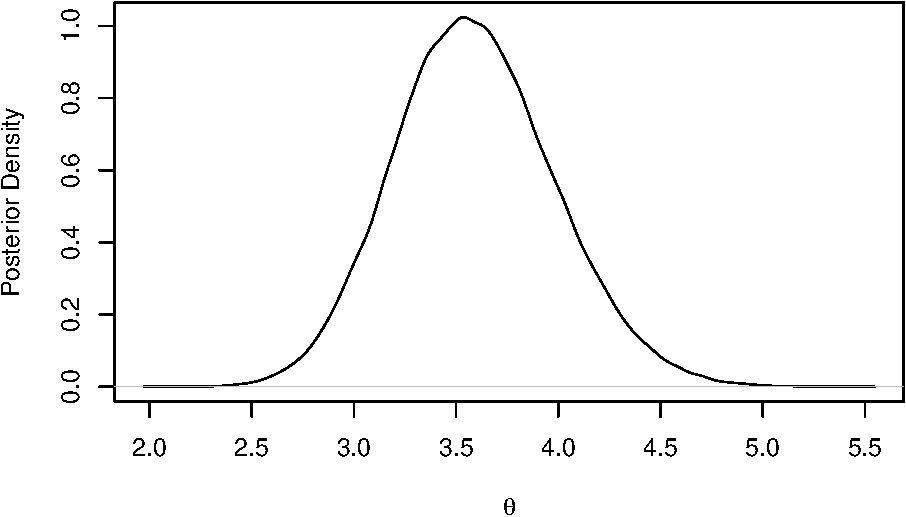
\includegraphics{hw7_files/figure-latex/unnamed-chunk-4-1.pdf}

Let's take a look at the \(p\)-values:

\begin{Shaded}
\begin{Highlighting}[]
\NormalTok{pvals}
\end{Highlighting}
\end{Shaded}

\begin{verbatim}
##     min     max   range    mean      sd 
## 0.00000 0.00165 0.53300 0.49690 0.55060
\end{verbatim}

The minimum and maximum are near zero, indicating that the model does
not fit the scale of the data well. However, the range, mean and
standard deviation fit well, indicating that while the model may not be
problematic, scaling the data and/or treating outliers might help. Below
is a plot that shows the observed values against the fitted ones:

\begin{Shaded}
\begin{Highlighting}[]
\NormalTok{Yp }\OtherTok{\textless{}{-}}\NormalTok{ sum\_airq}\SpecialCharTok{$}\NormalTok{statistics[}\FunctionTok{paste0}\NormalTok{(}\StringTok{"Yp["}\NormalTok{, }\DecValTok{1}\SpecialCharTok{:}\DecValTok{111}\NormalTok{, }\StringTok{"]"}\NormalTok{), }\DecValTok{1}\NormalTok{]}

\CommentTok{\# normal model}
\NormalTok{lin }\OtherTok{\textless{}{-}} \FunctionTok{lm}\NormalTok{(Y }\SpecialCharTok{\textasciitilde{}}\NormalTok{ X[,}\SpecialCharTok{{-}}\DecValTok{1}\NormalTok{])}

\FunctionTok{plot}\NormalTok{(Yp, Y, }\AttributeTok{xlab =} \FunctionTok{TeX}\NormalTok{(}\StringTok{"$Y\_p$"}\NormalTok{))}
\FunctionTok{abline}\NormalTok{(}\AttributeTok{a =} \DecValTok{0}\NormalTok{, }\AttributeTok{b =} \DecValTok{1}\NormalTok{, }\AttributeTok{lty =} \DecValTok{2}\NormalTok{)}
\end{Highlighting}
\end{Shaded}

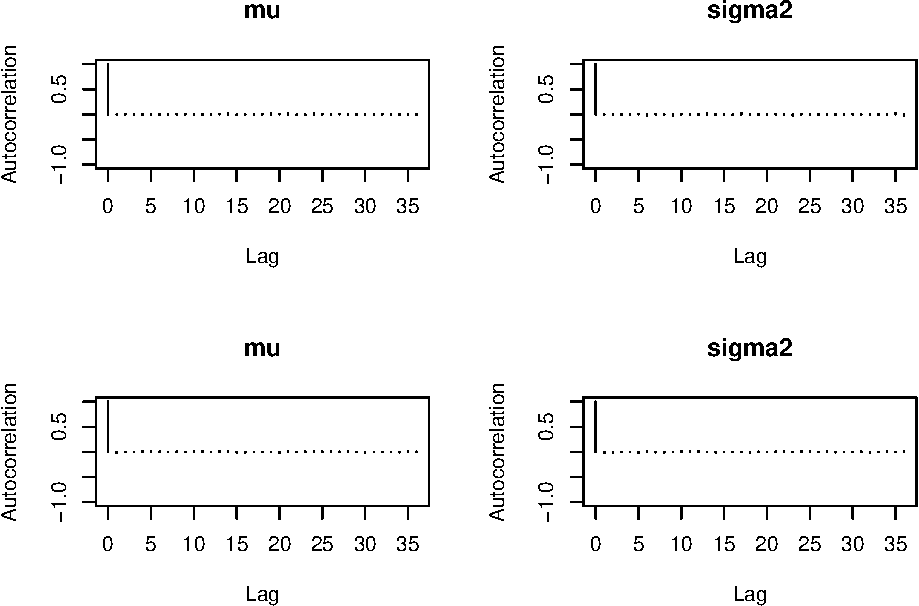
\includegraphics{hw7_files/figure-latex/unnamed-chunk-6-1.pdf}

It seems the model underfits the data at the extremes. This may because
of the scale of the reponse, shown in the below histogram:

\begin{Shaded}
\begin{Highlighting}[]
\FunctionTok{hist}\NormalTok{(Y)}
\end{Highlighting}
\end{Shaded}

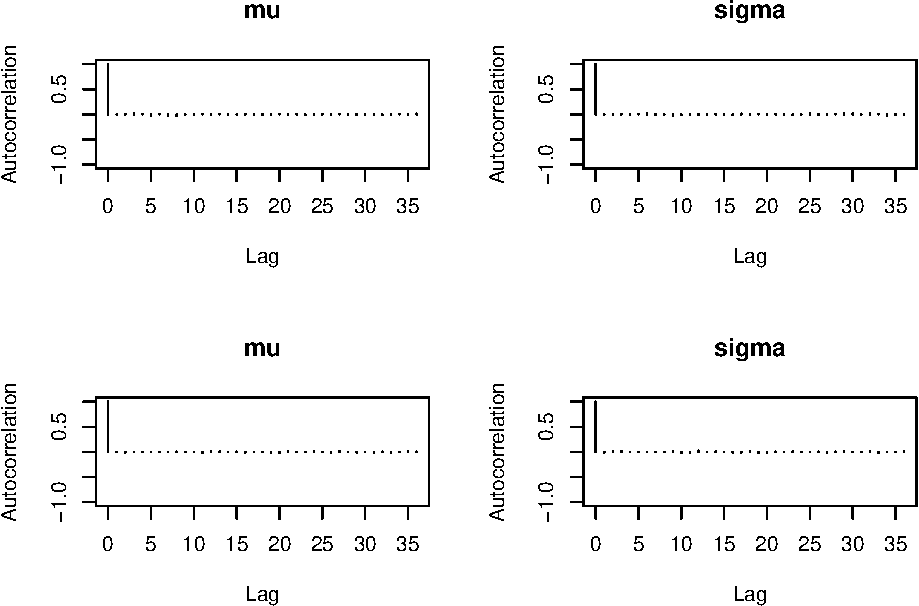
\includegraphics{hw7_files/figure-latex/unnamed-chunk-7-1.pdf}

Log transforming the response is a potential response to the faults
uncovered in the posterior predictive checks. Aside from this, the model
is good. The plot below shows :

\begin{Shaded}
\begin{Highlighting}[]
\CommentTok{\# residual plots for normal model}
\FunctionTok{par}\NormalTok{(}\AttributeTok{mfrow =} \FunctionTok{c}\NormalTok{(}\DecValTok{2}\NormalTok{, }\DecValTok{2}\NormalTok{), }\AttributeTok{font.main =} \DecValTok{1}\NormalTok{)}
\FunctionTok{plot}\NormalTok{(lin}\SpecialCharTok{$}\NormalTok{resid, }\AttributeTok{ylab =} \StringTok{"Residuals"}\NormalTok{, }\AttributeTok{main =} \StringTok{"Normal model"}\NormalTok{)}
\FunctionTok{abline}\NormalTok{(}\AttributeTok{h =} \DecValTok{0}\NormalTok{, }\AttributeTok{lty =} \DecValTok{2}\NormalTok{)}
\FunctionTok{plot}\NormalTok{(}\FunctionTok{hat}\NormalTok{(X), }\AttributeTok{ylab =} \StringTok{"Leverages"}\NormalTok{, }\AttributeTok{main =} \StringTok{"Normal model"}\NormalTok{)}
\FunctionTok{abline}\NormalTok{(}\AttributeTok{h =} \DecValTok{2} \SpecialCharTok{*}\NormalTok{ p }\SpecialCharTok{/}\NormalTok{ n, }\AttributeTok{lty =} \DecValTok{2}\NormalTok{)}

\CommentTok{\# linear model with log{-}transformed response}
\NormalTok{lin }\OtherTok{\textless{}{-}} \FunctionTok{lm}\NormalTok{(}\FunctionTok{log}\NormalTok{(Y) }\SpecialCharTok{\textasciitilde{}}\NormalTok{ X[,}\SpecialCharTok{{-}}\DecValTok{1}\NormalTok{])}
\NormalTok{pred\_lin }\OtherTok{\textless{}{-}} \FunctionTok{predict}\NormalTok{(lin, }\FunctionTok{data.frame}\NormalTok{(X[,}\SpecialCharTok{{-}}\DecValTok{1}\NormalTok{]))}

\CommentTok{\# plot the residuals}
\FunctionTok{plot}\NormalTok{(lin}\SpecialCharTok{$}\NormalTok{resid, }\AttributeTok{ylab =} \StringTok{"Residuals"}\NormalTok{, }\AttributeTok{main =} \StringTok{"log(Y) model"}\NormalTok{)}
\FunctionTok{abline}\NormalTok{(}\AttributeTok{h =} \DecValTok{0}\NormalTok{, }\AttributeTok{lty =} \DecValTok{2}\NormalTok{)}
\FunctionTok{plot}\NormalTok{(}\FunctionTok{hat}\NormalTok{(X), }\AttributeTok{ylab =} \StringTok{"Leverages"}\NormalTok{, }\AttributeTok{main =} \StringTok{"log(Y) model"}\NormalTok{)}
\FunctionTok{abline}\NormalTok{(}\AttributeTok{h =} \DecValTok{2} \SpecialCharTok{*}\NormalTok{ p }\SpecialCharTok{/}\NormalTok{ n, }\AttributeTok{lty =} \DecValTok{2}\NormalTok{)}
\end{Highlighting}
\end{Shaded}

\includegraphics{hw7_files/figure-latex/unnamed-chunk-8-1.pdf}

\begin{Shaded}
\begin{Highlighting}[]
\FunctionTok{par}\NormalTok{(}\AttributeTok{mfrow =} \FunctionTok{c}\NormalTok{(}\DecValTok{1}\NormalTok{, }\DecValTok{2}\NormalTok{), }\AttributeTok{font.main =} \DecValTok{1}\NormalTok{)}
\FunctionTok{plot}\NormalTok{(Y, Yp, }\AttributeTok{xlab =} \StringTok{"Y"}\NormalTok{, }\AttributeTok{ylab =} \StringTok{"Predicted value"}\NormalTok{, }\AttributeTok{main =} \StringTok{"Normal model"}\NormalTok{)}
\FunctionTok{abline}\NormalTok{(}\AttributeTok{a =} \DecValTok{0}\NormalTok{, }\AttributeTok{b =} \DecValTok{1}\NormalTok{)}
\FunctionTok{plot}\NormalTok{(}\FunctionTok{log}\NormalTok{(Y), pred\_lin, }\AttributeTok{xlab =} \StringTok{"log(Y)"}\NormalTok{, }\AttributeTok{ylab =} \StringTok{"Predicted value"}\NormalTok{, }\AttributeTok{main =} \StringTok{"log(Y) model"}\NormalTok{)}
\FunctionTok{abline}\NormalTok{(}\AttributeTok{a =} \DecValTok{0}\NormalTok{, }\AttributeTok{b =} \DecValTok{1}\NormalTok{)}
\end{Highlighting}
\end{Shaded}

\includegraphics{hw7_files/figure-latex/unnamed-chunk-8-2.pdf}

The transformation seemingly diminishes the discrepancy between the
fitted and observed data. The largest residual in the \(\log(Y)\) model
is due to the data point being equal to one, and thus \(\log(Y) = 0\)
which ends up far from the other observations.

\subsection{Exercise 2}\label{exercise-2}

We use the `'Mr October'' data (Section 2.4) \(Y_1 = 563\),
\(N_1 = 2820\), \(Y_2 = 10\) and \(N_2 = 27\). Compare the two models

\[
\begin{align*}
    &\mathcal M_1: Y_1 | \lambda_1 \sim \mathrm{Poisson}(N_1\lambda_1) \quad \text{and} \quad 
     Y_2 | \lambda_2 \sim \mathrm{Poisson}(N_2\lambda_2) \\
    &\mathcal M_2: Y_1 | \lambda_0 \sim \mathrm{Poisson}(N_1\lambda_0) \quad \text{and} \quad        
     Y_2 | \lambda_0 \sim \mathrm{Poisson}(N_2\lambda_0)
\end{align*}
\]

using Bayes factors, DIC and WAIC. Assume the \(\text{Uniform}(0, c)\)
prior for all \(\lambda_j\) and compare the results for \(c = 1\) and
\(c = 10\).

\subsubsection{Solution}\label{solution-1}

To recap briefly, the data are the total number of games played and
number of home runs in regular-season games as well as world series for
the American baseball player Reggie Jackson (``Mr.~October'').

We denote by \(Y_1\) and \(N_1\) the number of home runs and total
number of games in the regular season. World series data are analogously
labelled \(Y_2\) and \(N_2\). In this exercise, we are competing two
models \(\mathcal{M}_1\) and \(\mathcal{M}_2\), where the first model
claims that the rate of home runs is different when the player is
competing in the World Series or Regular-Season. The latter model claims
that there is no difference. Since we will be repeating the same
analyses quite a bit, it is convenient to declare a function which
automates this process.

\begin{Shaded}
\begin{Highlighting}[]
\CommentTok{\# Mr. October data}
\NormalTok{N }\OtherTok{\textless{}{-}} \FunctionTok{c}\NormalTok{(}\DecValTok{2820}\NormalTok{, }\DecValTok{27}\NormalTok{)}
\NormalTok{Y }\OtherTok{\textless{}{-}} \FunctionTok{c}\NormalTok{(}\DecValTok{563}\NormalTok{,  }\DecValTok{10}\NormalTok{)}

\CommentTok{\# Model parameters}
\NormalTok{p  }\OtherTok{\textless{}{-}} \DecValTok{2}
\NormalTok{n  }\OtherTok{\textless{}{-}} \DecValTok{2}

\CommentTok{\# Model strings}
\NormalTok{str\_october\_1 }\OtherTok{\textless{}{-}} \StringTok{"model\{}
\StringTok{  for (i in 1:n) \{}
\StringTok{    Y[i]     \textasciitilde{} dpois(N[i] * lambda[i])}
\StringTok{    like[i] \textless{}{-} dpois(Y[i], N[i] * lambda[i])}
\StringTok{  \}}
\StringTok{  }
\StringTok{  for (j in 1:p) \{ lambda[j] \textasciitilde{} dunif(0, c) \}}
\StringTok{\}"}

\NormalTok{str\_october\_2 }\OtherTok{\textless{}{-}} \StringTok{"model\{}
\StringTok{  for (i in 1:n) \{}
\StringTok{    Y[i]     \textasciitilde{} dpois(N[i] * lambda)}
\StringTok{    like[i] \textless{}{-} dpois(Y[i], N[i] * lambda)}
\StringTok{  \}}
\StringTok{  }
\StringTok{  lambda \textasciitilde{} dunif(0, c)}
\StringTok{\}"}

\NormalTok{models\_october }\OtherTok{\textless{}{-}} \FunctionTok{c}\NormalTok{(str\_october\_1, str\_october\_2)}

\CommentTok{\# Custom print function for information criterion}
\NormalTok{print\_ic }\OtherTok{\textless{}{-}} \ControlFlowTok{function}\NormalTok{(IC, P) \{}
  \ControlFlowTok{if}\NormalTok{(}\FunctionTok{class}\NormalTok{(IC) }\SpecialCharTok{==} \StringTok{"mcarray"}\NormalTok{) \{ }
\NormalTok{    IC }\OtherTok{\textless{}{-}} \FunctionTok{sum}\NormalTok{(IC)}
\NormalTok{    P  }\OtherTok{\textless{}{-}} \FunctionTok{sum}\NormalTok{(P)}
\NormalTok{  \}}
  \FunctionTok{cat}\NormalTok{(}\FunctionTok{paste}\NormalTok{(}\StringTok{"{-} Mean deviance     :"}\NormalTok{, }\FunctionTok{signif}\NormalTok{(IC, }\DecValTok{3}\NormalTok{), }\StringTok{"}\SpecialCharTok{\textbackslash{}n}\StringTok{"}\NormalTok{))}
  \FunctionTok{cat}\NormalTok{(}\FunctionTok{paste}\NormalTok{(}\StringTok{"{-} Penalty           :"}\NormalTok{, }\FunctionTok{signif}\NormalTok{(P, }\DecValTok{3}\NormalTok{), }\StringTok{"}\SpecialCharTok{\textbackslash{}n}\StringTok{"}\NormalTok{))}
  \FunctionTok{cat}\NormalTok{(}\FunctionTok{paste}\NormalTok{(}\StringTok{"{-} Penalised deviance:"}\NormalTok{, }\FunctionTok{signif}\NormalTok{(IC }\SpecialCharTok{+}\NormalTok{ P, }\DecValTok{3}\NormalTok{), }\StringTok{"}\SpecialCharTok{\textbackslash{}n}\StringTok{"}\NormalTok{)) }\CommentTok{\# LAGA}
\NormalTok{\}}

\CommentTok{\# Automates modelling process}
\NormalTok{mcmc\_october }\OtherTok{\textless{}{-}} \ControlFlowTok{function}\NormalTok{(model\_no, c) \{}
\NormalTok{  init\_october }\OtherTok{\textless{}{-}} \FunctionTok{textConnection}\NormalTok{(models\_october[model\_no])}

\NormalTok{  data }\OtherTok{\textless{}{-}} \FunctionTok{list}\NormalTok{(}\AttributeTok{N =}\NormalTok{ N, }\AttributeTok{Y =}\NormalTok{ Y, }\AttributeTok{c =}\NormalTok{ c, }\AttributeTok{n =}\NormalTok{ n, }\AttributeTok{p =}\NormalTok{ p)}
  \ControlFlowTok{if}\NormalTok{ (model\_no }\SpecialCharTok{==} \DecValTok{2}\NormalTok{) data }\OtherTok{\textless{}{-}}\NormalTok{ data[}\SpecialCharTok{{-}}\DecValTok{5}\NormalTok{]}

\NormalTok{  model\_october }\OtherTok{\textless{}{-}} \FunctionTok{jags.model}\NormalTok{(init\_october, }\AttributeTok{data =}\NormalTok{ data, }
                              \AttributeTok{n.chains =} \DecValTok{2}\NormalTok{, }\AttributeTok{quiet =} \ConstantTok{TRUE}\NormalTok{)}

  \FunctionTok{update}\NormalTok{(model\_october, }\AttributeTok{n.iter =} \FloatTok{1e+4}\NormalTok{, }\AttributeTok{progress.bar =} \StringTok{"none"}\NormalTok{)}

\NormalTok{  DIC     }\OtherTok{\textless{}{-}} \FunctionTok{dic.samples}\NormalTok{(model\_october, }\AttributeTok{n.iter =} \FloatTok{5e+4}\NormalTok{, }\AttributeTok{progress.bar =} \StringTok{"none"}\NormalTok{)}
  
\NormalTok{  samples }\OtherTok{\textless{}{-}} \FunctionTok{coda.samples}\NormalTok{(model\_october, }\AttributeTok{variable.names =} \FunctionTok{c}\NormalTok{(}\StringTok{"like"}\NormalTok{),}
                          \AttributeTok{n.iter =} \FloatTok{2e+4}\NormalTok{, }\AttributeTok{progress.bar =} \StringTok{"none"}\NormalTok{)}
  
  
\NormalTok{  like  }\OtherTok{\textless{}{-}} \FunctionTok{rbind}\NormalTok{(samples[[}\DecValTok{1}\NormalTok{]], samples[[}\DecValTok{2}\NormalTok{]])}
\NormalTok{  L\_bar }\OtherTok{\textless{}{-}} \FunctionTok{colMeans}\NormalTok{(like)}

\NormalTok{  Pw }\OtherTok{\textless{}{-}} \FunctionTok{sum}\NormalTok{(}\FunctionTok{apply}\NormalTok{(}\FunctionTok{log}\NormalTok{(like), }\DecValTok{2}\NormalTok{, var))}
\NormalTok{  WAIC }\OtherTok{\textless{}{-}} \SpecialCharTok{{-}}\DecValTok{2} \SpecialCharTok{*} \FunctionTok{sum}\NormalTok{(}\FunctionTok{log}\NormalTok{(L\_bar)) }\SpecialCharTok{+} \DecValTok{2} \SpecialCharTok{*}\NormalTok{ Pw}
  
  \FunctionTok{cat}\NormalTok{(}\FunctionTok{paste0}\NormalTok{(}\StringTok{"MODEL: "}\NormalTok{, model\_no, }\StringTok{", C: "}\NormalTok{, c, }\StringTok{"}\SpecialCharTok{\textbackslash{}n}\StringTok{"}\NormalTok{))}
  \FunctionTok{cat}\NormalTok{(}\StringTok{"==========================}\SpecialCharTok{\textbackslash{}n}\StringTok{"}\NormalTok{)}
  \FunctionTok{cat}\NormalTok{(}\StringTok{"WAIC}\SpecialCharTok{\textbackslash{}n}\StringTok{"}\NormalTok{)}
  \FunctionTok{print\_ic}\NormalTok{(WAIC, Pw)}
  \FunctionTok{cat}\NormalTok{(}\StringTok{"}\SpecialCharTok{\textbackslash{}n}\StringTok{"}\NormalTok{)}
  \FunctionTok{cat}\NormalTok{(}\StringTok{"DIC}\SpecialCharTok{\textbackslash{}n}\StringTok{"}\NormalTok{)}
  \FunctionTok{print\_ic}\NormalTok{(DIC}\SpecialCharTok{$}\NormalTok{deviance, DIC}\SpecialCharTok{$}\NormalTok{penalty)}
  \FunctionTok{cat}\NormalTok{(}\StringTok{"==========================}\SpecialCharTok{\textbackslash{}n\textbackslash{}n}\StringTok{"}\NormalTok{)}
\NormalTok{\}}
\end{Highlighting}
\end{Shaded}

Running the above function for the models \(\mathcal{M}_1\) and
\(\mathcal{M}_2\) with \(c = 1\) yields the result shown below:

\begin{Shaded}
\begin{Highlighting}[]
\FunctionTok{mcmc\_october}\NormalTok{(}\AttributeTok{model\_no =} \DecValTok{1}\NormalTok{, }\AttributeTok{c =} \DecValTok{1}\NormalTok{)}
\end{Highlighting}
\end{Shaded}

\begin{verbatim}
## MODEL: 1, C: 1
## ==========================
## WAIC
## - Mean deviance     : 15.8 
## - Penalty           : 1.02 
## - Penalised deviance: 16.8 
## 
## DIC
## - Mean deviance     : 14.3 
## - Penalty           : 2.01 
## - Penalised deviance: 16.4 
## ==========================
\end{verbatim}

\begin{Shaded}
\begin{Highlighting}[]
\FunctionTok{mcmc\_october}\NormalTok{(}\AttributeTok{model\_no =} \DecValTok{2}\NormalTok{, }\AttributeTok{c =} \DecValTok{1}\NormalTok{)}
\end{Highlighting}
\end{Shaded}

\begin{verbatim}
## MODEL: 2, C: 1
## ==========================
## WAIC
## - Mean deviance     : 17.2 
## - Penalty           : 0.571 
## - Penalised deviance: 17.8 
## 
## DIC
## - Mean deviance     : 16.4 
## - Penalty           : 0.992 
## - Penalised deviance: 17.4 
## ==========================
\end{verbatim}

Judging from the above output \(\mathcal{M}_1\) seems to be the slightly
favoured model, since both the \(\textit{DIC}\) and \(\textit{WAIC}\)
agree.

\begin{Shaded}
\begin{Highlighting}[]
\NormalTok{BF }\OtherTok{\textless{}{-}} \ControlFlowTok{function}\NormalTok{(Y1, Y2, c) \{}
\NormalTok{  numer }\OtherTok{\textless{}{-}}\NormalTok{ c }\SpecialCharTok{*} \FunctionTok{gamma}\NormalTok{(Y1 }\SpecialCharTok{+}\NormalTok{ Y2 }\SpecialCharTok{+} \DecValTok{2}\NormalTok{)}
\NormalTok{  denom }\OtherTok{\textless{}{-}} \FunctionTok{gamma}\NormalTok{(Y1 }\SpecialCharTok{+} \DecValTok{1}\NormalTok{) }\SpecialCharTok{*} \FunctionTok{gamma}\NormalTok{(Y2 }\SpecialCharTok{+} \DecValTok{1}\NormalTok{) }\SpecialCharTok{*} \DecValTok{2}\SpecialCharTok{\^{}}\NormalTok{(Y1 }\SpecialCharTok{+}\NormalTok{ Y2 }\SpecialCharTok{+} \DecValTok{1}\NormalTok{)}
  \FunctionTok{return}\NormalTok{(numer }\SpecialCharTok{/}\NormalTok{ denom)}
\NormalTok{\}}
\end{Highlighting}
\end{Shaded}

We encounter a problem evaluating this numerically\ldots{}

\subsection{Exercise 3}\label{exercise-3}

Download the \texttt{WWWusage} dataset in \texttt{R}. Using the data
from times \(t = 5, \ldots, 100\) as outcomes (earlier times may be used
as covariates), fit the autoregressive model

\[
\mathcal M_\ell: Y_t | Y_{t - 1}, \ldots, Y_1 \sim \text{Normal}(\beta_0 + \beta_1 Y_{t - 1} + \cdots \beta_\ell Y_{t - \ell}, \sigma^2)
\]

where \(Y_t\) is the WWW usage at time \(t\). Compare the models
\(\mathcal M_\ell\) with \(\ell = 1, 2, 3, 4\) and select the best time
lag \(\ell\).

\subsubsection{Solution}\label{solution-2}

\begin{Shaded}
\begin{Highlighting}[]
\FunctionTok{data}\NormalTok{(WWWusage)}
\FunctionTok{plot}\NormalTok{(WWWusage)}
\end{Highlighting}
\end{Shaded}

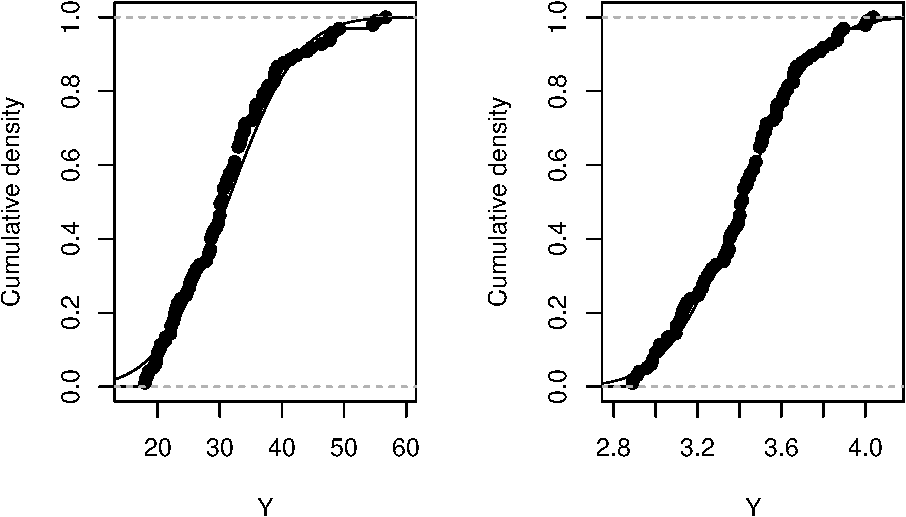
\includegraphics{hw7_files/figure-latex/unnamed-chunk-12-1.pdf}

Pretty. Define a function to fit an autoregressive model
\(\mathcal M_\ell\) where the lag time \(\ell\) enters as an input
parameter:

\begin{Shaded}
\begin{Highlighting}[]
\NormalTok{Y }\OtherTok{\textless{}{-}}\NormalTok{ WWWusage}
\NormalTok{n }\OtherTok{\textless{}{-}} \FunctionTok{length}\NormalTok{(Y)}

\NormalTok{autoreg\_model }\OtherTok{\textless{}{-}} \ControlFlowTok{function}\NormalTok{(l) \{}
\NormalTok{  data }\OtherTok{\textless{}{-}} \FunctionTok{list}\NormalTok{(}\AttributeTok{Y =}\NormalTok{ Y, }\AttributeTok{l =}\NormalTok{ l, }\AttributeTok{n =}\NormalTok{ n)}
  
\NormalTok{  autoreg\_init }\OtherTok{\textless{}{-}} \FunctionTok{textConnection}\NormalTok{(}\StringTok{"model\{}
\StringTok{    for (t in 5:n) \{}
\StringTok{      Y[t]     \textasciitilde{} dnorm(alpha + inprod(beta, Y[t{-}1:l]), tau)}
\StringTok{      like[t] \textless{}{-} dnorm(Y[t], alpha + inprod(beta, Y[t{-}1:l]), tau)}
\StringTok{    \}}
\StringTok{    }
\StringTok{    alpha \textasciitilde{} dnorm(0, 0.001)}
\StringTok{    tau   \textasciitilde{} dgamma(0.1, 0.1)}
\StringTok{    for (j in 1:l) \{ beta[j] \textasciitilde{} dnorm(0, 0.001) \}}
\StringTok{    }
\StringTok{  \}"}\NormalTok{)}
  
\NormalTok{  model\_autoreg }\OtherTok{\textless{}{-}} \FunctionTok{jags.model}\NormalTok{(autoreg\_init, }\AttributeTok{data =}\NormalTok{ data, }\AttributeTok{n.chains =} \DecValTok{2}\NormalTok{, }\AttributeTok{quiet =} \ConstantTok{TRUE}\NormalTok{)}
  \FunctionTok{update}\NormalTok{(model\_autoreg, }\FloatTok{1e+4}\NormalTok{, }\AttributeTok{progress.bar =} \StringTok{"none"}\NormalTok{)}
  
\NormalTok{  samples }\OtherTok{\textless{}{-}} \FunctionTok{coda.samples}\NormalTok{(model\_autoreg, }\AttributeTok{variable.names =} \FunctionTok{c}\NormalTok{(}\StringTok{"like"}\NormalTok{), }\AttributeTok{n.iter =} \FloatTok{2e+4}\NormalTok{,}
                          \AttributeTok{progress.bar =} \StringTok{"none"}\NormalTok{)}

\NormalTok{  DIC }\OtherTok{\textless{}{-}} \FunctionTok{dic.samples}\NormalTok{(model\_autoreg, }\AttributeTok{n.iter =} \FloatTok{5e+4}\NormalTok{, }\AttributeTok{progress.bar =} \StringTok{"none"}\NormalTok{)}
  
\NormalTok{  like  }\OtherTok{\textless{}{-}} \FunctionTok{rbind}\NormalTok{(samples[[}\DecValTok{1}\NormalTok{]], samples[[}\DecValTok{2}\NormalTok{]])}
\NormalTok{  L\_bar }\OtherTok{\textless{}{-}} \FunctionTok{colMeans}\NormalTok{(like)}
\NormalTok{  Pw    }\OtherTok{\textless{}{-}} \FunctionTok{sum}\NormalTok{(}\FunctionTok{apply}\NormalTok{(}\FunctionTok{log}\NormalTok{(like), }\DecValTok{2}\NormalTok{, var))}
\NormalTok{  WAIC }\OtherTok{\textless{}{-}} \SpecialCharTok{{-}}\DecValTok{2} \SpecialCharTok{*} \FunctionTok{sum}\NormalTok{(}\FunctionTok{log}\NormalTok{(L\_bar)) }\SpecialCharTok{+} \DecValTok{2} \SpecialCharTok{*}\NormalTok{ Pw}
\NormalTok{\}}

\NormalTok{aut\_1 }\OtherTok{\textless{}{-}} \FunctionTok{autoreg\_model}\NormalTok{(}\DecValTok{1}\NormalTok{)}
\NormalTok{aut\_2 }\OtherTok{\textless{}{-}} \FunctionTok{autoreg\_model}\NormalTok{(}\DecValTok{2}\NormalTok{)}
\NormalTok{aut\_3 }\OtherTok{\textless{}{-}} \FunctionTok{autoreg\_model}\NormalTok{(}\DecValTok{3}\NormalTok{)}
\NormalTok{aut\_4 }\OtherTok{\textless{}{-}} \FunctionTok{autoreg\_model}\NormalTok{(}\DecValTok{4}\NormalTok{)}
\end{Highlighting}
\end{Shaded}


\end{document}
